\documentclass[a4paper,12pt]{article}

\usepackage{a4wide}
\usepackage{amsmath}
\usepackage{amssymb}
\usepackage{amsthm}
\usepackage[czech]{babel}
\usepackage{bookmark}
\usepackage{enumerate}
\usepackage[T1]{fontenc}
\usepackage{forest}
\usepackage{hyperref}
\usepackage[utf8]{inputenc}
\usepackage{lmodern}
\usepackage{multicol}
\usepackage{tikz}

\theoremstyle{definition}
    \newtheorem{problem}{Příklad}

% \theoremstyle{remark}
%     \newtheorem*{steps}{Postup řešení}

\theoremstyle{plain}
    \newtheorem*{solution}{Řešení}
    

\DeclareRobustCommand\proves{\mathrel{|}\joinrel\mkern-.5mu\mathrel{-}}
\DeclareMathOperator{\Conseq}{Csq}
\DeclareMathOperator{\M}{M}

% hide solutions
\newif\ifhidesolutions
    \hidesolutionstrue
    % \hidesolutionsfalse

\ifhidesolutions
    \usepackage{environ}
    \NewEnviron{hide}{}
    \let\solution\hide
    \let\endsolution\endhide
\fi









\begin{document}

\section*{NAIL062 V\&P Logika: Druhý domácí  úkol}
% predikátová logika bez rezoluce

\subsubsection*{Termín odevzdání: 18. 12. v 10:40.}
Celkem 10 bodů. Řešení odevzdejte v papírové podobě na cvičení nebo, pokud nebudete moci přijít, emailem před začátkem cvičení. Řešení musí být rozumně čitelné, a v případě odevzdání emailem musí mít bílé pozadí. Je zakázáno o úkolech až do termínu odevzdání jakýmkoliv způsobem komunikovat s kýmkoliv kromě mne. Řešení musí být 100\% vaší vlastní prací, a je vaší povinností zajistit, že nikdo nebude mít přístup k vašemu řešení.

\bigskip

\noindent {\textbf{Poznámka:} Používáte-li tablo metodu, musí řešení obsahovat tablo korektně sestrojené přesně podle definice: nedělejte žádné zkratky, nevynechávejte vrcholy nad rámec konvence z přednášky, apod. Podobně, používáte-li rezoluční metodu, musí řešení obsahovat korektní rezoluční strom. (Rezoluční důkaz zapisovat nemusíte.) 

Úkol neobsahuje rezoluci v predikátové logice, protože ji teprve budeme cvičit. V zápočtovém testu se ale velmi pravděpodobně vyskytne.

\medskip\begin{problem}[4 body]
    Uvažte následující tvrzení:
    \begin{enumerate}[label=(\roman*)]\it
        \item Každý docent napsal alespoň jednu učebnici.
        \item Každou učebnici napsal nějaký docent.
        \item U každého docenta někdo studuje.
        \item Každý, kdo studuje u nějakého docenta, přečetl všechny učebnice od tohoto docenta.
        \item Každou učebnici někdo přečetl.
    \end{enumerate}    
    \begin{enumerate}
    \item Formalizujte tvrzení (i)--(v) po řadě jako \underline{sentence} $\varphi_1,\varphi_2,\varphi_3,\varphi_4,\varphi_5$ v predikátové logice v jazyce $L=\langle N, S, P, D, U\rangle$ bez rovnosti, kde $N,S,P$ jsou binární relační symboly ($N(x,y)$ znamená ``$x$ napsal $y$'', $S(x,y)$ znamená ``$x$ studuje u $y$'', $P(x,y)$ znamená ``$x$ přečetl $y$'') a $D,U$ jsou unární relační symboly (``být docentem'', ``být učebnicí''). {\it (2b)}
    \item Sestrojte dokončené tablo z teorie $T=\{\varphi_1,\varphi_2,\varphi_3,\varphi_4\}$ s položkou $F\varphi_5$ v kořeni. {\it (3b)}
    \item Je sentence $\varphi_5$ pravdivá v teorii $T$? Je lživá v $T$? Je nezávislá v $T$? Zdůvodněte. {\it (1b)}
    \item Má teorie $T$ kompletní konzervativní extenzi? Zdůvodněte. {\it (2b)}
    \item Uvažme teorii $T'=T\cup \{D(x),S(x,y),P(x,y)\}$. Kolik má teorie $T'$ dvouprvkových modelů (až na izomorfismus)? Zdůvodněte. {\it (2b)}
    \end{enumerate}
\end{problem}



\medskip\begin{problem}[3 body]  
    Známe následující informace o zadávání zakázek:
    \begin{enumerate}[label=(\roman*)] \it
        \item Každý úředník, který je odpovědný za nějakou zakázku a vezme od nějaké společnosti úplatek, je kriminálník.
        \item Zakázku vyhraje pouze společnost, která podplatí všechny úředníky odpovědné za tuto zakázku.
        \item Pan Lubor je úředník.
        \item Nějaká společnost vyhrála nějakou zakázku, za kterou je pan Lubor odpovědný.
    \end{enumerate}
    Pomocí rezoluce dokažte, že: {\it (v) Pan Lubor je kriminálník.}
    \begin{enumerate}
        \item Uvedená tvrzení vyjádřete \underline{sentencemi} $\varphi_1, \dots, \varphi_5$ v jazyce $L=\langle U, Z, S, K, P, V, O, l \rangle$ bez rovnosti, kde $U, Z, S$ a $K$ jsou unární relační symboly a $U(x), Z(x), S(x), K(x)$ znamenají (po řadě) ``$x$ je úředník / zakázka / společnost / kriminálník'', $P, V, O$ jsou binární relační symboly, kde $P(x,y), V(x,y), O(x,y)$ značí (po řadě) ``$x$ podplatil $y$'', ``$x$ vyhrál $y$'' a ``$x$ je odpovědný za $y$'' a $l$ je konstanta označující pana Lubora.
        \item Pomocí skolemizace předchozích formulí nebo jejich negací nalezněte otevřenou teorii $T$ (případně ve větším jazyce), která je nesplnitelná, právě když  $\{\varphi_1, \varphi_2, \varphi_3, \varphi_4\} \models \varphi_5$.
        \item Převedením axiomů $T$ do CNF nalezněte teorii $T'$ ekvivalentní $T$ a axiomatizovanou klauzulemi. Napište $T'$ v množinové reprezentaci.
        
        \bigskip

        \textbf{Části (d) a (e) nebudou hodnoceny, zkuste si sami až procvičíme rezoluci:}
        \item Rezolucí dokažte, že $T'$ není splnitelná. Rezoluční zamítnutí znázorněte rezolučním stromem. U každého kroku uveďte použitou unifikaci.
        \item Nalezněte konjunkci základních instancí axiomů $T'$, která je nesplnitelná.
    \end{enumerate}
\end{problem}


\medskip\begin{problem}[2 body]
    Nechť $T=\{R(x,x),\ R(x,y) \wedge R(y,x) \to x=y,\ R(x,y) \wedge R(y,z) \to R(x,z),\ R(x,y) \vee R(y,x), \neg c=d, \varphi,\psi\}$ je teorie jazyka $L=\langle R,P,f,c,d\rangle$ s rovností, kde $R$, $P$ jsou binární relační symboly, $f$ je binární funkční symbol, $c$, $d$ jsou konstantní symboly  
    a $\varphi$, $\psi$ jsou následující formule:
    \begin{align*}
        \varphi:\quad P(x,y) &\leftrightarrow R(x,y) \wedge \neg x=y\\
        \psi:\quad P(x,y) &\to P(x,f(x,y)) \wedge P(f(x,y),y)
    \end{align*}
    \begin{enumerate}
        \item Najděte expanzi struktury $\langle \mathbb{Q},\le \rangle$ (v jazyce $L'=\langle R\rangle$) do jazyka $L$ na model teorie~$T$.
        \item Je sentence $(\forall x)R(c,x)$ pravdivá/lživá/nezávislá v $T$? Zdůvodněte všechny tři odpovědi.
        \item Nalezněte dvě neekvivalentní kompletní jednoduché extenze $T$ nebo zdůvodněte, proč neexistují.
        \item Nechť $T'=T\setminus\{\varphi,\psi\}$ je jazyka $L'=\langle R,f,c,d\rangle$. Je teorie $T$ extenzí teorie $T'$? Je teorie $T$ konzervativní extenzí teorie $T'$? Uveďte zdůvodnění.
    \end{enumerate}
\end{problem}


\medskip\begin{problem}[1 bod]
    Nechť $T=\{(\exists x)R(x), (\exists y)\neg P(x,y), (\exists y)(\forall z)(\neg R(x)\vee P(y,z))\}$ je teorie jazyka $L=\langle P,R\rangle$ bez rovnosti. Najděte otevřenou teorii $T'$ ekvisplnitelnou s $T$. Převeďte $T'$ do CNF a výslednou formuli $S$ zapište v množinové reprezentaci.
\end{problem}


\end{document}





% \medskip\begin{problem}[4 body]
%     Nechť $T$ je teorie jazyka $L=\langle T \rangle$ s rovností, kde $T$ je ternární relační symbol, s axiomy:
%     \begin{align*}
%         T(x,y,z)&\to x\ne y \wedge y\ne z \wedge x\ne z \\
%         T(x,y,z)&\to T(y,x,z)\wedge T(y,z,x)\wedge T(z,y,x)\wedge T(z,x,y)\wedge T(x,z,y)\\
%         x\ne y &\to (\exists z)(T(x,y,z)\wedge(\forall u)(T(x,y,u)\to u=z))
%     \end{align*}
%     Modely teorie $T$ jsou tzv. \emph{Steinerovy systémy trojic}, v našem případě uspořádaných. Uvažme model $\mathcal{F}=\langle \{1,2,\dots,7\},T^F\rangle$ teorie $T$ na obrázku (tzv. \emph{Fanova rovina}), kde každá ``přímka'' reprezentuje trojici prvků, jež jsou v relaci $T^F$ v libovolném pořadí, tedy $T^F=\{(2,4,6),(6,2,4),\dots\}$.
%     \begin{center}
%         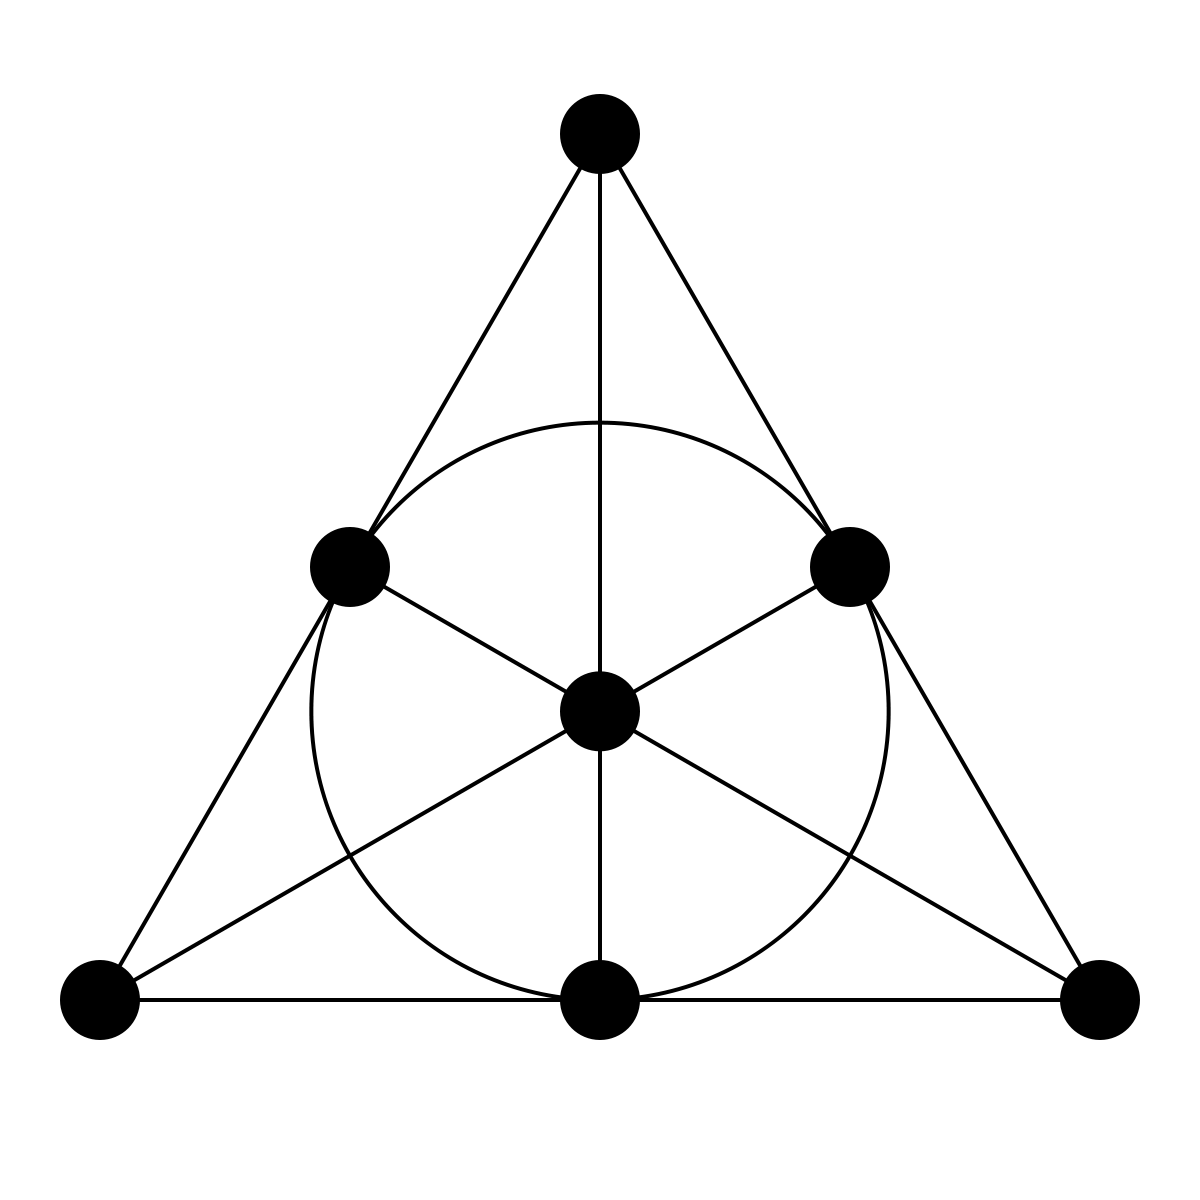
\includegraphics[height=4cm]{files/fano.png}  
%     \end{center}
%     \begin{enumerate}        
%         \item Nalezněte co nejmenší množinu parametrů $A$, která v modelu $\mathcal{F}$ umožňuje definovat libovolný jeho prvek (formulí jazyka $L$). Pro každý prvek napište příslušnou definující formuli (s dosazenými parametry). Zdůvodněte, proč je $A$ nejmenší možná.
%         \item Jsou teorie $T'=T \cup \{f(x,y)=z \leftrightarrow T(x,y,z)\}$ a $T''=T\cup \{f(x,y)=z \leftrightarrow T(x,y,z) \vee (x=y \wedge y=z)\}$, kde $f$ je nový binární funkční symbol, (korektními) extenzemi teorie $T$ o definici? Uveďte zdůvodnění.
%     \end{enumerate} 
% \end{problem}




